\documentclass[11pt,twoside]{article}
\usepackage{techrep-PFG-ic}
\usepackage[english]{babel}
\usepackage[utf8]{inputenc}
\usepackage{amsmath}
\usepackage{amssymb}
\usepackage{array}
\usepackage{caption}
\usepackage{float}

\DeclareMathOperator*{\E}{\mathbb{E}}
\DeclareMathOperator*{\argmax}{\arg\!\max}

\newcommand{\subsubsubsection}[1]{\paragraph{#1}\mbox{}\\}
\setcounter{secnumdepth}{4}
\setcounter{tocdepth}{4}

\begin{document}

%%% PÁGINA DE CAPA %%%%%%%%%%%%%%%%%%%%%%%%%%%%%%%%%%%%%%%%%%%%%%%

% Número do relatório
\TRNumber{13} 

% DATA DE PUBLICAÇÃO (PARA A CAPA)
%
\TRYear{18}  % Dois dígitos apenas
\TRMonth{07} % Numérico, 01-12

% LISTA DE AUTORES PARA CAPA (sem afiliações).
\TRAuthor{Guilherme Bueno Andrade \and Andre Rodrigues Oliveira \and Zanoni Dias}

% TÍTULO PARA A CAPA (use \\ para forçar quebras de linha).
\TRTitle{Sorting Permutations by Reversals and Transpositions with Reinforcement Learning}

\TRMakeCover

\markboth{Andrade, Oliveira and Dias}{Sorting Permutations with RL}
\pagestyle{myheadings}

\title{Sorting Permutations by Reversals and Transpositions\\ with Reinforcement Learning}

\newcommand*\samethanks[1][\value{footnote}]{\footnotemark[#1]}
\author{Guilherme Bueno Andrade\thanks{gbuenoandrade@gmail.com} \and
Andre Rodrigues Oliveira\thanks{Institute of Computing, University of Campinas, Brazil.} \and Zanoni Dias\samethanks}

\date{}

\maketitle

%%%%%%%%%%%%%%%%%%%%%%%%%%%%%%%%%%%%%%%%%%%%%%%%%%%%%%%%%%%%%%%%%%%%%%

\begin{abstract} 

Finding the minimum number of mutations necessary for one genome to transform into another is a major problem in molecular biology. This problem can be reduced to sorting a permutation using certain operations, where, in this work, the operations considered are reversals and transpositions. We present two different approaches using reinforcement learning to address that. Our results show that this approach is competitive when the permutations are small. However, converging gets trickier as $|p|$ grows larger.

\end{abstract}

\section{Introduction}

Finding the minimum number of mutations necessary for one genome to transform into another using certain operations, a concept usually referred to as \textit{distance} between genomes, is a major problem in molecular biology. Two common operations are reversals and transpositions. A reversal happens when a fragment of the DNA filament gets reversed in the final replica, and a transposition when two fragments of DNA change places. 

Formally, in this work we treat a genome of size $n$ as being equal to a permutation $p$ of integers from $0$ to $n$. Also, a reversal operation $f_r(i,j)$ applied to permutation $p = (p_0\ \ldots\ p_{i-1}\ p_{i}\ \ldots\ p_{j}\ \ldots\ p_{n-1})$ generates $p \cdot f_r(i,j) = (p_0\ \ldots\ p_{i-1}\ p_{j}\ \ldots\ p_{i}\ \ldots\ p_{n-1})$. Similarly, a transposition operation $f_t(i,j,k)$ applied to\\ $p = (p_0\ \ldots\ p_{i-1}\ p_{i}\ \ldots\ p_{j}\ p_{j+1}\ \ldots\ p_{k}\ p_{k+1}\ \ldots\ p_{n-1})$ generates\\ $p \cdot f_t(i,j,k) = (p_0\ \ldots\ p_{i-1}\ p_{j+1}\ \ldots\ p_{k}\ p_{i}\ \ldots\ p_{j}\ p_{k+1}\ \ldots\ p_{n-1})$. Finally, the distance $d(p, q)$ between permutations $p$ and $q$ is equal to the minimum number of operations needed to transform $p$ into $q$.

It can be shown that finding $d(p, q)$ is equivalent to the problem of finding the distance between some permutation $\alpha$ and the identity permutation $\iota$ [ref]. Furthermore, Caprara (1999) proved that this problem is NP-Hard [ref]. That being so, this work proposes using Reinforcement Learning to come up with a heuristic for finding $d(p, \iota)$ for any arbitrary permutation $p$.

\section{Reinforcement Learning}

% https://medium.freecodecamp.org/an-introduction-to-reinforcement-learning-4339519de419

\subsection{Overview}

Reinforcement Learning (RL), like other branches of Machine Learning, has been drawing a lot of attention from the community in the recent years. Google DeepMind's AlphaGo victory over Lee Sedol~\cite{googlelee} - world champion of the game Go, is one of many examples of recent astonishing applications of the technique. It is based an agent learning how to accomplish a certain goal based on interactions with the environment.

RL can be thought of as a sequence of episodes. Each of which consists of the agent initially at an initial state $S_0$. Then, based on a policy $\pi$, where a policy is a function that maps states to actions, it takes an action $a$, ending up at state $S_1$ and receiving some reward $R_1$. This process keeps going until the agent reaches a terminal state. Its goal is to find a function $\pi*$, known as optimal policy, that maximizes the cumulative discounted reward:

\begin{gather}
	G(t) = \sum_{\tau = 0}^{\infty} \gamma ^ {\tau} R_{t + \tau + 1}
	,
\intertext{Where:}
	\begin{tabular}{>{$}r<{$}@{\ :\ }l}
		\gamma \in [0,1) & is a discount rate to highlight most likely short-term rewards
	\end{tabular}\nonumber
\end{gather}

\subsection{Exploitation vs. Exploration}
 
A major concern in RL is the exploitation/explorarion trade-off. Exploration is about exploring new possibilities within the environment and finding out more information about it. Exploitation, on the other hand, is related to exploiting already known information so as to maximize the total reward. 

Initially, the agent has no other option but to randomly explore the environment; however, as it learns about its surroundings, it can fall into the trap of sticking to safe known actions and miss larger rewards that depend on exploring unknown states.

This work uses the Epsilon-greedy strategy to address that problem. It specifies an exploration rate $\epsilon$, which is set to 1 initially. This rate definies the ratio of the steps that will be done randomly. Before selecting an action, the agent generates a random number $x$. If $x > \epsilon$, then it will select the best known action (exploit); otherwise, it will select an action at random (explore). As the agent acquires more knowledge about the environment, $\epsilon$ is progressively reduced.

\subsection{Q-table and the Bellman Equation}

In value-based RL, the branch being considered in this work, the efforts are concentraded on maximizing the value function $V_\pi$:

\begin{equation}
	V_\pi(s) = \mathbb{E}_{\pi} [G(t)\ |\ S_t = s]
\end{equation}

It tells the agent the expected future reward it will get at each state. $V_\pi$ can be generalized so as to also include actions, which is known as Q-table:

\begin{equation} \label{qtable}
	Q^\pi(s, a) = \mathbb{E}_{\pi} [G(t)\ |\ S_t = s,\ A_t = a]
\end{equation}

The previous definition is convenient because it allows the agent to pick the best action that can be performed from state $s$ by simply finding $\operatorname*{arg\,max}_{a} Q^\pi(s,a)$.

Furthermore, $Q$ can be expressed in terms of itself. An expression known as the Bellman Equation [ref]:

\begin{gather}\label{bellman}
	Q^\pi(s, a) = \mathbb{E}_{\pi} [R_{t+1} + \gamma \sum_{a'} Q^\pi(s', a')]
	,
\intertext{Where:}
	\begin{tabular}{>{$}r<{$}@{\ :\ }l}
		s' & is the state reached after action $a$ is taken from state $s$ \\
		a' & is an action that can be taken from $s'$
	\end{tabular}\nonumber
\end{gather}

The above form can be used alongside dynamic programming to develop iterative approaches to solve the problem [ref].

\subsection{Function Approximation}

If one can calculate the Q-table from equation \ref{qtable}, they could trivially come up with a great policy. At each state $s$, the agent should simply be greedy and select the action $a$ that maximizes $Q^\pi(s, a)$. As mentioned in the last section, finding the Q-table can be easily done with dynamic programming.

However, as the number of states grows largers, dynamic programming and other iterative approaches become unfeasible due to our computers' memory and time limitations. Fortunately, it turns out that the Q-table can be approximated instead of having its exact values determined, and it will still produce great results [ref]. This work tries to achieve that using both linear regression and deep neural networks.

\subsection{Monte Carlo and Temporal Difference Learning}

In Monte Carlo Approaches, the agent plays an entire episode, keeping track of the rewards received at each timestep so it can calculate the cumulative discounted reward. After that, it updates the value function for each visited stated based on the expression [ref]:

\begin{gather}
	V(S_t) \leftarrow V(S_t) + \alpha [G(t) - V(S_t)]
	,
\intertext{Where:}
	\begin{tabular}{>{$}r<{$}@{\ :\ }l}
		\alpha & is the learning rate
	\end{tabular}\nonumber
\end{gather}

Therefore, the agent only learns after an entire episode has been played. In Temporal Diference Learning, however, the value of $V$ is updated after each timestep. At time $t+1$, the observations made during time $t$ are already being considered. In its simplest form, the method is called TD(0) or 1-step TD, and its update equation is as follows:

\begin{equation} \label{td0}
	V(S_t) \leftarrow V(S_t) + \alpha [R_{t+1} + \gamma V(S_{t+1}) - V(S_t)]
\end{equation}

The right-hand side of the previous equation is referred to as the TD(0) error.

\subsection{TD-Lambda}
% https://amreis.github.io/ml/reinf-learn/2017/11/02/reinforcement-learning-eligibility-traces.html

TD(0) is biased as it relies on information from a single timestep to perform its updates. It does not take into account the fact that the action that caused a reward might have happened several timesteps earlier, which can lead to slow convergence [ref]. Monte Carlo methods, although not biased, have a lot of variance since they use the rewards of an entire episode in order to perform updates [ref].

To address that, from equation \ref{td0}, we can define the 1-step return, $G_t^{(1)} = R_{t+1} + \gamma V(S_{t+1})$. We can extend the concept further to 2-step return, $G_t^{(2)} = R_{t+1} + \gamma R_{t+2} + \gamma^2 V(S_{t+2})$, and, generically, to, $G_t^{(n)} = R_{t+1} + \gamma R_{t+2} + \ldots + \gamma^n V(S_{t+n})$. 

TD-Lambda methods use a mathematical trick to average all the possible n-step returns into a single one. This is done by introducing a factor $\lambda \in [0, 1]$ and weighting the nth-return with $\gamma^{n-1}$. It can be shown [ref] that when $\lambda = 0$, the method is equivalent to TD(0), and when $\lambda = 1$, equivalent to Monte Carlo. So, intuitively, by setting $0 < \lambda < 1$, we can get a mixture of both methods [ref].

\subsection{Q-learning}

Q-learning is another technique based on Temporal Difference Learning to learn the Q-table. The main difference between it and the previous shown techniques is that Q-learning is off-policy, while TD(0) and TD-Lambda are on-policy [ref]. This is reflected in its update equation, derived from the Bellman Equation [ref]:

\begin{equation} \label{qlearning}
	Q(s, a) \leftarrow Q(s, a) + \alpha [R_{t+1} + \gamma \max_{a'} Q(s', a') - Q(s,a)]
\end{equation}

The fact that there is no constraint regarding the action $a'$, only that it must optimizes $Q$, makes it an off-policy method [ref].

\subsubsection{Deep Q-learning}

% https://storage.googleapis.com/deepmind-data/assets/papers/DeepMindNature14236Paper.pdf
% https://arxiv.org/abs/1509.06461
% https://jaromiru.com/2016/11/07/lets-make-a-dqn-double-learning-and-prioritized-experience-replay/
% Watkins Ch. and Dayan P. – Q-learning, Machine Learning 8, 1992 q learning convergence\
% https://jaromiru.com/2016/09/27/lets-make-a-dqn-theory/#fnref-38-6

In order to approximate the Q-table to make using it feasible even when the number of states is very large, since Google AlphaGo's paper [ref], it has becoming common the use of a deep neural network. Even though standard Q-learning is proven to converge when there are finite states and each pair state-action is presented repeatedly [ref], the same proof does not hold when neural networks are being used to calculate $Q$. To face with this issue, this work makes use of several ideas found in the literature [ref] to stabilize the training. They are presented in the following subsections.

\subsubsection{Experience Replay}\label{experience}

During each step of an episode, our estimation can be shifted according to equation \ref{qlearning}. It is reasonable to think that as more truth is being introduced into the system, it will eventually converge; however, this is often not true. One of the reasons is that samples arrive in order they are experienced and as such are highly correlated. Also, by throwing away our samples immediately after we use it, we are not extracting all the knowledge they carry.

Experience replay address that by storing samples into a queue and during each learning step, it samples a random batch and performs gradient descend on it. As samples get old, they are gradually discarded.

\subsubsection{Target Network}

The points $Q(s, a)$ and $Q(s', a')$ in equation \ref{qlearning} are very close together as $s'a$ is a state reachable from $s$. That being so, updates to one of them influence the other, which in turn can lead to instabilities.

To overcome that, a second network, called target network, can be used to provide more stable $\widetilde{Q}$ values. This second network is a mery copy of the first one; however, it does not get updated every simulation step. Instead, it stays frozen in time, and only after several steps it is updated by copying the weights from the first network. The introduction of the target network changes our update equation to the following:

\begin{equation} \label{new_qlearning}
	Q(s, a) \leftarrow Q(s, a) + \alpha [R_{t+1} + \gamma \max_{a'}\widetilde{Q}(s', a') - Q(s,a)]
\end{equation}


\subsubsection{Double Learning}\label{double_learning}

Due to the $\max$ term presented in both equations \ref{qlearning} and \ref{new_qlearning}, the approximation tends to overstimate the Q function value, which can severely impact on stability of the algorithm [ref]. A solution proposed by Hado van Hasselt (2010) [ref], called Double Learning, consists of two Q functions, $Q_1$ and $Q_2$, that are independently learned. One function is then used to determine the maximizing action and second to estimate its value. As we are already making use of two different networks, Hado van Hasselt's approach can be easily introduced to the update equation \ref{new_qlearning}. Its augmented version is as follows:

\begin{equation}\label{double_equation}
	Q(s, a) \leftarrow Q(s, a) + \alpha [R_{t+1} + \gamma \widetilde{Q}(s', \argmax_{a'}{Q(s', a')}) - Q(s,a)]
\end{equation}


\section{Experiment}

\subsection{Modeling}

\subsubsection{State Representation}

Three different state representations were considered. They are as follows.

\begin{itemize}
	\item \textit{One-Hot Encoding}: Each number is treaded as a category. By doing so, each $p$ is mapped to a matrix $m$, where $m_{ij} = 1$ if $p_i = j$, and $0$ otherwise. 
	\item \textit{Min-Max Normalization}: $P$ is mapped to an array $v$,\\ where $v_i = p_i / (|p| - 1)$.
	\item \textit{Permutation Characterization}: $p$ is mapped to an array $v$ of $30$ features, where the features are the ones described in the work by Flavio (2017) [ref].
\end{itemize}

\subsubsection{Proposed Architecture}

The experiment was based on two different architectures. The first one consisted of a Double Deep Q-Network (DDQN), with a main network and a secondary target network. Also, it included both experience replay (see \ref{experience}) and double learning (see \ref{double_learning}) optimizations.

Both main and secondary networks used the following architecture:

\begin{table}[H]
	\begin{center}
		\begin{tabular}{|c|c|c|c|} 
			\hline
			Layer & Number of Units & Activation & Type \\
			\hline\hline
			Input layer & - & - & - \\ 
			\hline
			Hidden layer 1 & 256 & ReLU & Fully-connected\\
			\hline
			Hidden layer 2 & 256 & ReLU & Fully-connected\\
			\hline
			Output layer & $|$Actions$|$ & Linear & Fully-connected\\
			\hline
		\end{tabular}
		\caption{Main and secondary networks architecture}
	\end{center}
\end{table}

Furthermore, the hyperparameters selected were as follows:

\begin{table}[H]
	\begin{center}
		\begin{tabular}{|c |c|} 
			\hline
			Hyperparameter & Value \\
			\hline\hline
			$\gamma$ & $0.99$ \\
			$\alpha$ & $0.001$ \\
			$|$Batch$|$ & $32$ \\
			$\epsilon_{min}$ & $0.1$ \\
			$\epsilon_{decay}$ & $0.993$ \\
			$|$Replay queue$|$ & 2000 \\
			Loss & logcosh \\
			Optimizer & Adam \\
			Step reward & $-1$ \\
			\hline
		\end{tabular}
		\caption{Hyperparameters used in the DDQN}
	\end{center}
\end{table}

Nevertheless, we tried a second different approach. An agent based on the TD-Lambda algorithm was also built. In order to approximate the Q-table, it relied on a much simpler linear regressor. Also, since $Q$ is highly nonlinear (see equation \ref{bellman}), the radial basis function kernel was used as a pre-processing step. The agent's hyperparameters were the following:

\begin{table}[H]
	\begin{center}
		\begin{tabular}{|c |c|} 
			\hline
			Hyperparameter & Value \\
			\hline\hline
			$\gamma$ & $0.999$ \\
			$\alpha$ & $0.01$ \\
			$\lambda$ & $0.25$ \\
			$\epsilon_{min}$ & $0.05$ \\
			$\epsilon_{decay}$ & $0.99$ \\
			RBF Components & $4$ \\
			RBF $\gamma$ array & $[5.0, 2.0, 1.0, 0.5]$ \\
			Step reward & $-1$ \\
			\hline
		\end{tabular}
		\caption{Hyperparameters used to implement TD-Lambda}
	\end{center}
\end{table}

\subsubsection{Speeding up the Convergence}

Despite being finite, the state space is still enormous given that it is in $\mathcal{O}(|p|!)$. Being that the case, several techniques were tried so as to decrease training time. The ones that seemed more promising are mentioned below:

\begin{itemize}
	\item \textit{Greedy Pre-Training}: Kececioglu and Sankoff (1995) [ref] presented a 2-approximation for sorting a permutation using reversals, its output is represented below:

	\begin{gather}\label{greedy}
		d(p) = (p,\ a(p),\ a'(a(p)),\ \ldots,\ \iota)
		,
	\intertext{Where:}
		\begin{tabular}{>{$}r<{$}@{\ :\ }l}
			a & is the resultant permutation after applying action $a$ on $p$ \\
			\iota & is the identity permutation
		\end{tabular}\nonumber
	\end{gather}

	From expression \ref{greedy}, let $\hat{V}$:
	\begin{equation}
		\hat{V}(s) = (\gamma^{|d(s)|} - 1) / (\gamma - 1)
	\end{equation}

	Furthermore, we can define function $\hat{Q}$, which can be shown to be lower bound on $Q$:

	\begin{gather}
		\hat{Q}(s, a) = -1 + \gamma \hat{V}(s')
		,
	\intertext{Where:}
		\begin{tabular}{>{$}r<{$}@{\ :\ }l}
			s' & is the state reached by taking action $a$ at state $s$
		\end{tabular}\nonumber
	\end{gather}

	Having defined those, we can talk about our pre-training strategy. It consisted of partially fitting our neural network and linear regressor to function $\hat{Q}$ before start learning from proper episodes.

\end{itemize}

\subsection{Results and Discussion}

The models were trained experiencing $10000$ episodes, each of which had $s_0$ set to a random permutation. After that, in order for the models to effectively sort a permutation $p$, the exploration rate $\epsilon$ was kept constant and equal to $0.2$, and then the models were run for another $100$ episodes, where $s_0$ was always equal to $p$. The best score among those simulations was considered the model's answer $\hat{d}(p, \iota)$. Finally, the performance ratio $\eta = \hat{d}(p, \iota) / d(p, \iota)$ was used to compare different configurations. The closer $\eta$ was to $1$, the better.

Based on $\eta$, it was found that one-hot encoding state representation was slightly better than our other different attempts (see figure \ref{chart:state}). Nonetheless, investigating more effective representations so as to lead to better generalizations is a pending task. Also, as expected, our DDQN agent presented much better results than the ones presented by our simpler one based on TD-Lambda algorithm (see figure \ref{chart:alg}).

\begin{figure}
\centering
\begin{minipage}{.5\textwidth}
  \centering
	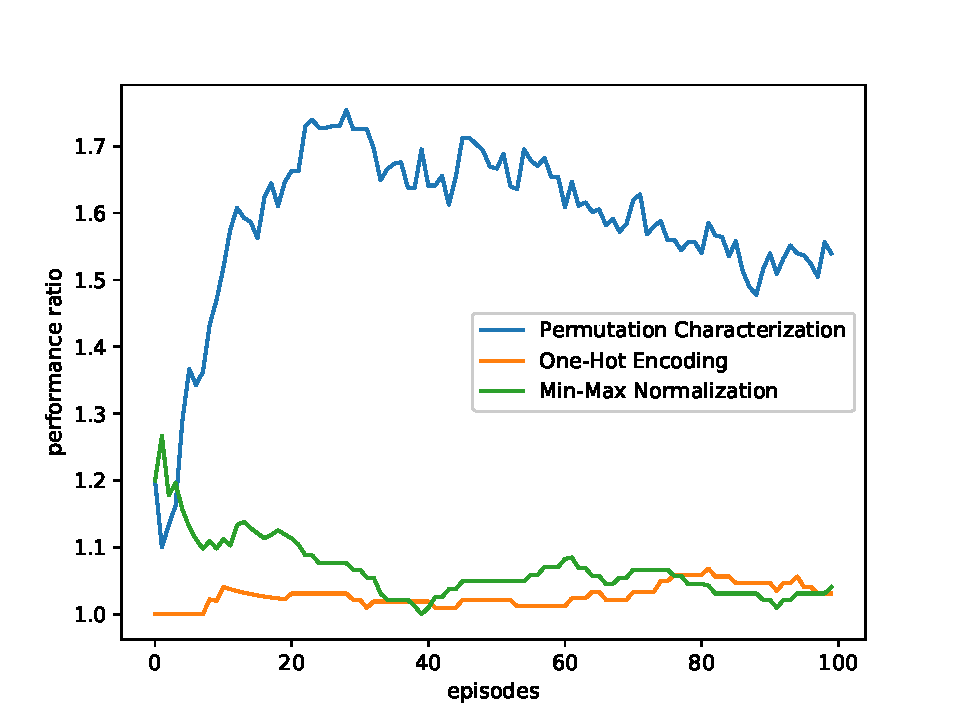
\includegraphics[scale=0.5]{charts/states_comp.pdf}
  \caption{Comparing different state represantions}
  \label{chart:state}
\end{minipage}%
\begin{minipage}{.5\textwidth}
  \centering
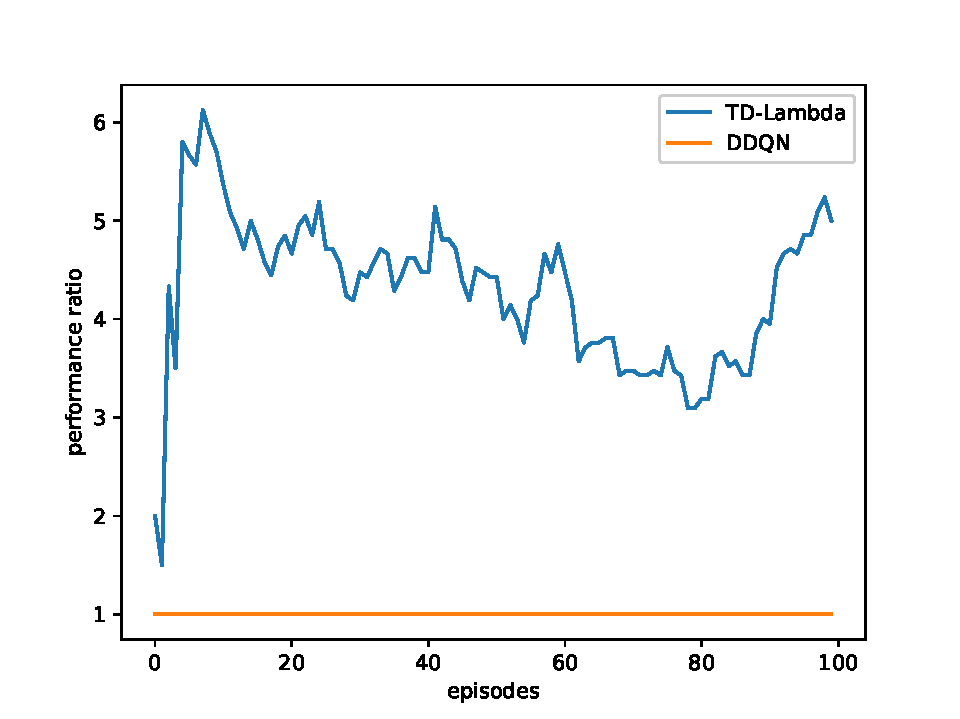
\includegraphics[scale=0.5]{charts/lambda_ddqn.pdf}
  \caption{Comparing different algorithms}
  \label{chart:alg}
\end{minipage}
\end{figure}

Having defined the best RL architecture based on the results above, we ran it against Kececioglu and Sankoff (1995)'s greedy approach. Our model consistently outperformed theirs when $|p| < 15$ (see figure \ref{chart:rl_greedy}). However, converging starts getting tricky and time-consuming as $|p|$ gets bigger. So, it is still early to define our approach as being \textit{practical}. 

\begin{figure}
	\begin{center}
		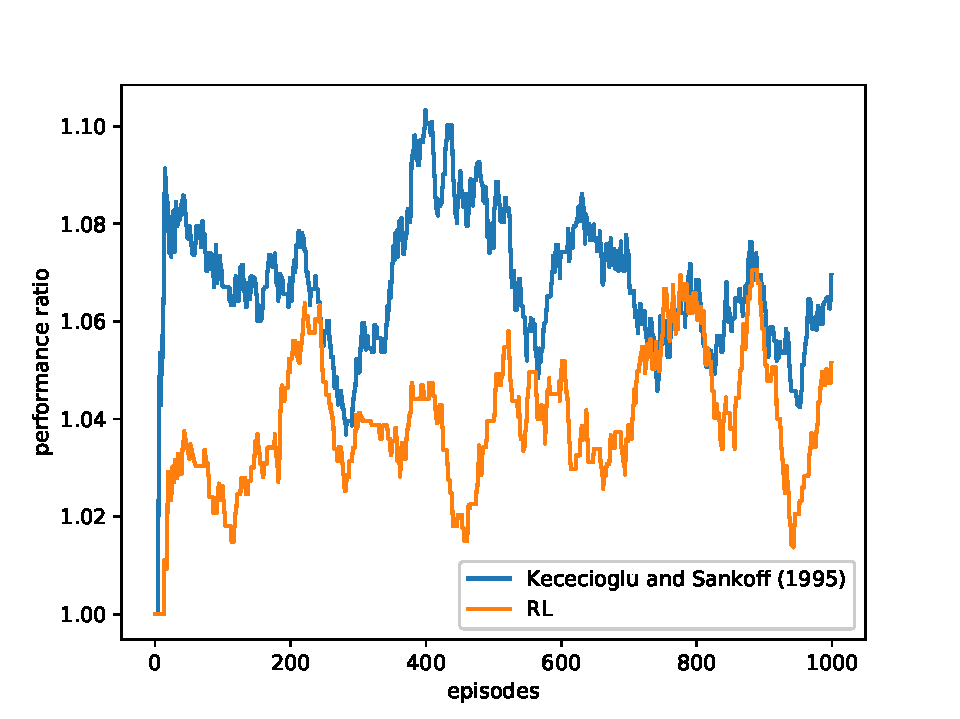
\includegraphics[scale=0.8]{charts/rl_greedy_comp.pdf}
		\caption{RL vs. Kececioglu and Sankoff's greedy approach}
		\label{chart:rl_greedy}

	\end{center}
\end{figure}

\bibliographystyle{abbrv}
\bibliography{main}

\end{document}
